\documentclass[12pt,a4paper,twoside,openright,titlepage,final]{article}
\usepackage{fontspec}
\usepackage{amsmath}
\usepackage{amsfonts}
\usepackage{amssymb}
\usepackage{makeidx}
\usepackage{graphicx}
\usepackage[hidelinks,unicode=true]{hyperref}
\usepackage[spanish,es-nodecimaldot,es-lcroman,es-tabla,es-noshorthands]{babel}
\usepackage[left=3cm,right=2cm, bottom=4cm]{geometry}
\usepackage{natbib}
\usepackage{microtype}
\usepackage{ifdraft}
\usepackage{verbatim}
\usepackage[obeyDraft]{todonotes}
\ifdraft{
	\usepackage{draftwatermark}
	\SetWatermarkText{BORRADOR}
	\SetWatermarkScale{0.7}
	\SetWatermarkColor{red}
}{}
\usepackage{booktabs}
\usepackage{longtable}
\usepackage{calc}
\usepackage{array}
\usepackage{caption}
\usepackage{subfigure}
\usepackage{footnote}
\usepackage{url}
\usepackage{tikz}

\setsansfont[Ligatures=TeX]{texgyreadventor}
\setmainfont[Ligatures=TeX]{texgyrepagella}

%*******************************************************
%                 NO MODIFICAR
\newcommand*{\FSfont}[1]{%
  \fontencoding{T1}\fontfamily{#1}\selectfont}

\newlength{\tpheight}\setlength{\tpheight}{0.9\textheight}
\newlength{\txtheight}\setlength{\txtheight}{0.9\tpheight}
\newlength{\tpwidth}\setlength{\tpwidth}{0.9\textwidth}
\newlength{\txtwidth}\setlength{\txtwidth}{0.9\tpwidth}
\newlength{\drop}
%*******************************************************

% Crea una portada con los siguientes parámetros
%
% #1 : Título 
% #2 : Subtítulo
% #3 : Subsubtítulo
% #4 : Autor(es)
% #5 : Lugar
%

\newcommand*{\portada}[5]{
\begin{titlepage}
\begingroup
\vspace*{1cm}
\drop = 0.2\txtheight
\centering
\vfill
{\Huge \scshape #1}\\[\baselineskip]
{\Large \textbf{#2}}\\[\baselineskip]
{\Large \scshape #3}\\[\baselineskip]
\vspace*{0.3cm}
{\large \textit{#4}}\\[0.5\drop]

\includegraphics[scale=0.35]{./imagenes/logoURJC.jpg}
\vspace*{1.5cm}

{\large \scshape #5, \today} \par
\begin{center}
\end{center}
\vfill\null
\endgroup
\end{titlepage}
}
 %*****************************************************
 


\author{José Ignacio Escribano}

\title{Caso práctico IV}

\setlength{\parindent}{0pt}

\begin{document}

\pagenumbering{alph}
\setcounter{page}{1}

\portada{Caso Práctico IV}{Modelización y tratamiento de la incertidumbre}{Modelos lineales}{José Ignacio Escribano}{Móstoles}

\listoffigures
\thispagestyle{empty}
\newpage

\tableofcontents
\thispagestyle{empty}
\newpage


\pagenumbering{arabic}
\setcounter{page}{1}

\section{Introducción}

Este caso práctico buscaremos un modelo lineal para predecir el valor medio de las casas ocupadas por los propietarios, a partir de trece variables como el crimen per cápita, la concentración de óxido nítrico, el número de medio de habitaciones por vivienda, entre otras. 

\section{Resolución del caso práctico}

En primer lugar, observamos el fichero de datos para ver qué variables son cuanitativas y categóricas. Observamos que todas las variables son cuantitativas, excepto una que es categórica: CHAS (1, si las vías cruzan el río y, 0 en caso contrario). Para cada de las variables, calculamos un resumen (mínimo, máximo, primer y tercer cuartil) usando R. El resumen de cada de las variables es el siguiente:

\begin{verbatim}
      CRIM               ZN             INDUS            CHAS        
  Min.   : 0.0060   Min.   :  0.00   Min.   : 0.46   Min.   :0.00000  
  1st Qu.: 0.0820   1st Qu.:  0.00   1st Qu.: 5.19   1st Qu.:0.00000  
  Median : 0.2565   Median :  0.00   Median : 9.69   Median :0.00000  
  Mean   : 3.6135   Mean   : 11.36   Mean   :11.14   Mean   :0.06917  
  3rd Qu.: 3.6770   3rd Qu.: 12.50   3rd Qu.:18.10   3rd Qu.:0.00000  
  Max.   :88.9760   Max.   :100.00   Max.   :27.74   Max.   :1.00000  
       NOX               RM             AGE              DIS        
  Min.   :0.3850   Min.   :3.561   Min.   :  2.90   Min.   : 1.130  
  1st Qu.:0.4490   1st Qu.:5.886   1st Qu.: 45.02   1st Qu.: 2.100  
  Median :0.5380   Median :6.208   Median : 77.50   Median : 3.208  
  Mean   :0.5547   Mean   :6.285   Mean   : 68.57   Mean   : 3.795  
  3rd Qu.:0.6240   3rd Qu.:6.623   3rd Qu.: 94.08   3rd Qu.: 5.189  
  Max.   :0.8710   Max.   :8.780   Max.   :100.00   Max.   :12.126  
       RAD              TAX           PTRATIO            B         
  Min.   : 1.000   Min.   :187.0   Min.   :12.60   Min.   :  0.32  
  1st Qu.: 4.000   1st Qu.:279.0   1st Qu.:17.40   1st Qu.:375.38  
  Median : 5.000   Median :330.0   Median :19.05   Median :391.44  
  Mean   : 9.549   Mean   :408.2   Mean   :18.46   Mean   :356.67  
  3rd Qu.:24.000   3rd Qu.:666.0   3rd Qu.:20.20   3rd Qu.:396.22  
  Max.   :24.000   Max.   :711.0   Max.   :22.00   Max.   :396.90  
      LSTAT            MEDV      
  Min.   : 1.73   Min.   : 5.00  
  1st Qu.: 6.95   1st Qu.:17.02  
  Median :11.36   Median :21.20  
  Mean   :12.65   Mean   :22.53  
  3rd Qu.:16.95   3rd Qu.:25.00  
  Max.   :37.97   Max.   :50.00  
\end{verbatim}

Al tener muchas variables, no podemos obtener mucha información sobre las variables a partir de estos datos, por lo que representamos el histograma de cada variable, que de forma gráfica, nos aportará más información que el resumen de cada variable (Figura~\ref{fig:histogramas}).\\


\begin{figure}[tbph!]
\centering
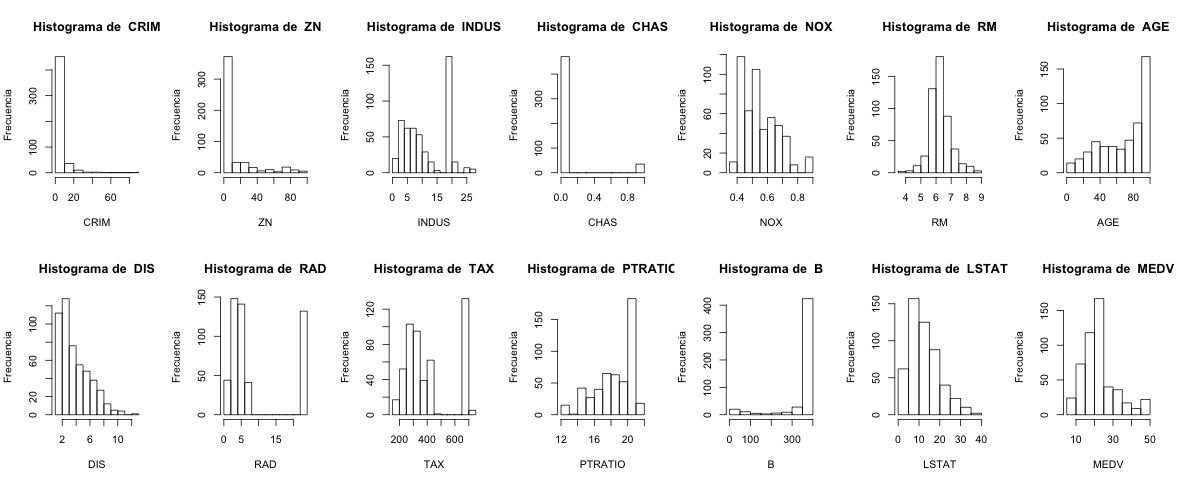
\includegraphics[width=0.9\linewidth]{imagenes/histogramas}
\caption{Histograma de cada una de las variables del conjunto de datos}
\label{fig:histogramas}
\end{figure}

Observamos que existen variables que tienen mucha asimetría como las variables CRIM, ZN, CHAS y B. Para estar convencidos totalmente, calculamos la asimetría de cada variable con R. Los datos se muestran a continuación:

\begin{table}[htbp!]
\centering
\begin{tabular}{@{}cc@{}}
\toprule
Variable & Asimetría \\ \midrule
CRIM     & 5.192     \\ \midrule
ZN       & 2.212     \\ \midrule
INDUS    & 0.293     \\ \midrule
CHAS     & 3.385     \\ \midrule
NOX      & 0.724     \\ \midrule
RM       & 0.401     \\ \midrule
AGE      & -0.595    \\ \midrule
DIS      & 1.005     \\ \midrule
RAD      & 0.998     \\ \midrule
TAX      & 0.665     \\ \midrule
PTRATIO  & -0.797    \\ \midrule
B        & -2.873    \\ \midrule
LSTAT    & 0.901     \\ \midrule
MEDV     & 1.101     \\ \bottomrule
\end{tabular}
\end{table}

Como sospechábamos, las variables CRIM, ZN, CHAS y B tienen una fuerte asimetría, por lo que transformamos cada variable aplicando logaritmos. A estas nuevas variables las llamamos LOGCRIM, LOGZN, LOGCHAS y LOGB.\\

En primer lugar usaremos un modelo sin transformaciones, es decir,

\begin{multline*}
E[MEDV_i |x, \theta] = \beta_0 + \beta_1 CRIM_i + \beta_2 ZN_i + \beta_3 INDUS_i + \beta_4 CHAS_i \\ + \beta_5 NOX_i + \beta_6 RM_i + \beta_7 AGE_i + \beta_8 DIS_i + \beta_9 RAD_i + \beta_{10} TAX_i + \beta_{11} PTRATIO_i \\ + \beta_{12} B_i + \beta_{13} LSTAT_i
\end{multline*}

El resumen de este modelo es el siguiente:

\begin{verbatim}
Residuals:
     Min       1Q   Median       3Q      Max 
-15.5940  -2.7295  -0.5179   1.7767  26.1987 

Coefficients:
              Estimate Std. Error t value Pr(>|t|)    
(Intercept)  3.646e+01  5.103e+00   7.144 3.28e-12 ***
CRIM        -1.080e-01  3.287e-02  -3.287 0.001087 ** 
ZN           4.642e-02  1.373e-02   3.381 0.000779 ***
INDUS        2.055e-02  6.150e-02   0.334 0.738352    
CHAS         2.687e+00  8.616e-01   3.119 0.001924 ** 
NOX         -1.777e+01  3.820e+00  -4.651 4.24e-06 ***
RM           3.810e+00  4.179e-01   9.116  < 2e-16 ***
AGE          6.915e-04  1.321e-02   0.052 0.958274    
DIS         -1.476e+00  1.995e-01  -7.398 6.01e-13 ***
RAD          3.060e-01  6.635e-02   4.613 5.07e-06 ***
TAX         -1.233e-02  3.760e-03  -3.280 0.001112 ** 
PTRATIO     -9.528e-01  1.308e-01  -7.283 1.31e-12 ***
B            9.311e-03  2.686e-03   3.467 0.000573 ***
LSTAT       -5.248e-01  5.072e-02 -10.347  < 2e-16 ***
---
Signif. codes:  0 ‘***’ 0.001 ‘**’ 0.01 ‘*’ 0.05 ‘.’ 0.1 ‘ ’ 1 

Residual standard error: 4.745 on 492 degrees of freedom
Multiple R-squared: 0.7406,	Adjusted R-squared: 0.7338 
F-statistic: 108.1 on 13 and 492 DF,  p-value: < 2.2e-16 
\end{verbatim}

Observamos que tenemos un coeficiente de determinación $R^2 = 0.7338$ que es bastante alto, pero probaremos haciendo alguna transformación a los datos para obtener un modelo mejor.\\

Si aplicamos al modelo las variables transformadas LOGCRIM, LOGZN, LOGCHAS y LOGB, el modelo de regresión lineal queda de la siguiente manera:

\begin{multline*}
E[MEDV_i |x, \theta] = \beta_0 + \beta_1 LOGCRIM_i + \beta_2 LOGZN_i + \beta_3 INDUS_i + \beta_4 LOGCHAS_i \\ + \beta_5 NOX_i + \beta_6 RM_i + \beta_7 AGE_i + \beta_8 DIS_i + \beta_9 RAD_i + \beta_{10} TAX_i + \beta_{11} PTRATIO_i \\ + \beta_{12} LOGB_i + \beta_{13} LSTAT_i
\end{multline*}

Al resolver este modelo con R, obtendremos un error puesto que las variables ZN y CHAS tienen elementos que son cero, por lo que $log(0) = -\infty$. No podemos aplicar esta tranformación a estas variables. El nuevo modelo, sin estas variables transformadas, queda de la siguiente forma:

\begin{multline*}
E[MEDV_i |x, \theta] = \beta_0 + \beta_1 LOGCRIM_i + \beta_2 ZN_i + \beta_3 INDUS_i + \beta_4 CHAS_i \\ + \beta_5 NOX_i + \beta_6 RM_i + \beta_7 AGE_i + \beta_8 DIS_i + \beta_9 RAD_i + \beta_{10} TAX_i + \beta_{11} PTRATIO_i \\ + \beta_{12} LOGB_i + \beta_{13} LSTAT_i
\end{multline*}

Si resolvemos con R este modelo se obtiene la siguiente información:

\begin{verbatim}
Residuals:
     Min       1Q   Median       3Q      Max 
-14.9955  -2.6666  -0.5467   1.6758  26.7270 

Coefficients:
              Estimate Std. Error t value Pr(>|t|)    
(Intercept)  36.736482   5.222405   7.034 6.74e-12 ***
LOGCRIM       0.402651   0.278326   1.447 0.148621    
ZN            0.047008   0.014145   3.323 0.000956 ***
INDUS         0.019971   0.062244   0.321 0.748459    
CHAS          2.835766   0.868064   3.267 0.001164 ** 
NOX         -18.495224   3.979490  -4.648 4.32e-06 ***
RM            3.849395   0.421452   9.134  < 2e-16 ***
AGE          -0.001863   0.013429  -0.139 0.889728    
DIS          -1.390883   0.199905  -6.958 1.11e-11 ***
RAD           0.189284   0.076145   2.486 0.013256 *  
TAX          -0.012084   0.003794  -3.185 0.001540 ** 
PTRATIO      -0.923299   0.132703  -6.958 1.11e-11 ***
B             0.010909   0.002719   4.013 6.94e-05 ***
LSTAT        -0.560681   0.051076 -10.977  < 2e-16 ***
---
Signif. codes:  0 ‘***’ 0.001 ‘**’ 0.01 ‘*’ 0.05 ‘.’ 0.1 ‘ ’ 1 

Residual standard error: 4.787 on 492 degrees of freedom
Multiple R-squared: 0.7361,	Adjusted R-squared: 0.7291 
F-statistic: 105.5 on 13 and 492 DF,  p-value: < 2.2e-16 
\end{verbatim}

Vemos que el coeficiente de determinación $R^2$ es menor que en el modelo anterior, por lo que este modelo con las variables transformadas es peor que el anterior.\\

Como último intento intentamos otra transformación. Para obtener un nuevo modelo, aplicamos lo visto en el ejemplo resuelto. Aplicamos una transformación logarítima a la variable dependeniente, MEDV. Esta nueva variable la llamaremos LOGMEDV.\\

El nuevo modelo es

\begin{multline*}
E[LOGMEDV_i |x, \theta] = \beta_0 + \beta_1 CRIM_i + \beta_2 ZN_i + \beta_3 INDUS_i + \beta_4 CHAS_i \\ + \beta_5 NOX_i + \beta_6 RM_i + \beta_7 AGE_i + \beta_8 DIS_i + \beta_9 RAD_i + \beta_{10} TAX_i \\ +  \beta_{11} PTRATIO_i + \beta_{12} B_i + \beta_{13} LSTAT_i
\end{multline*}

Resolvemos el modelo con R, y el resumen es el siguiente:

\begin{verbatim}
Coefficients:
              Estimate Std. Error t value Pr(>|t|)    
(Intercept)  4.1020911  0.2042738  20.081  < 2e-16 ***
CRIM        -0.0102716  0.0013155  -7.808 3.52e-14 ***
ZN           0.0011724  0.0005495   2.134 0.033358 *  
INDUS        0.0024666  0.0024614   1.002 0.316794    
CHAS         0.1008924  0.0344857   2.926 0.003596 ** 
NOX         -0.7784407  0.1528904  -5.091 5.07e-07 ***
RM           0.0908326  0.0167279   5.430 8.87e-08 ***
AGE          0.0002106  0.0005287   0.398 0.690614    
DIS         -0.0490883  0.0079834  -6.149 1.62e-09 ***
RAD          0.0142670  0.0026556   5.372 1.20e-07 ***
TAX         -0.0006257  0.0001505  -4.157 3.80e-05 ***
PTRATIO     -0.0382727  0.0052365  -7.309 1.10e-12 ***
B            0.0004136  0.0001075   3.847 0.000135 ***
LSTAT       -0.0290353  0.0020299 -14.304  < 2e-16 ***
---
Signif. codes:  0 ‘***’ 0.001 ‘**’ 0.01 ‘*’ 0.05 ‘.’ 0.1 ‘ ’ 1 

Residual standard error: 0.1899 on 492 degrees of freedom
Multiple R-squared: 0.7896,	Adjusted R-squared: 0.7841 
F-statistic: 142.1 on 13 and 492 DF,  p-value: < 2.2e-16 
\end{verbatim}

Este nuevo modelo mejora al anterior: el anterior tenía $R^2 = 0.7338$ y, este nuevo, $R^2 = 0.7841$. Observamos que casi todas las variables son influyentes, salvo INDUS y AGE, que apenas aportan al modelo. Por brevedad, consideraremos cuatro variables como las más influyentes (las que tienen un p-valor menor) de este modelo que son LSTAT (porcentaje de clase baja), PTRATIO (ratio alumno-profesor), DIS (distancia ponderada a cinco centros de empleo) y CRIM (crimen per cápita).\\

Para cada de las cuatro variables más influyentes, representamos el diagrama de dispersión con respecto al valor de las casas (MEDV)(Figura~\ref{fig:variables_relevantes}).

\begin{figure}[tbph!]\centering
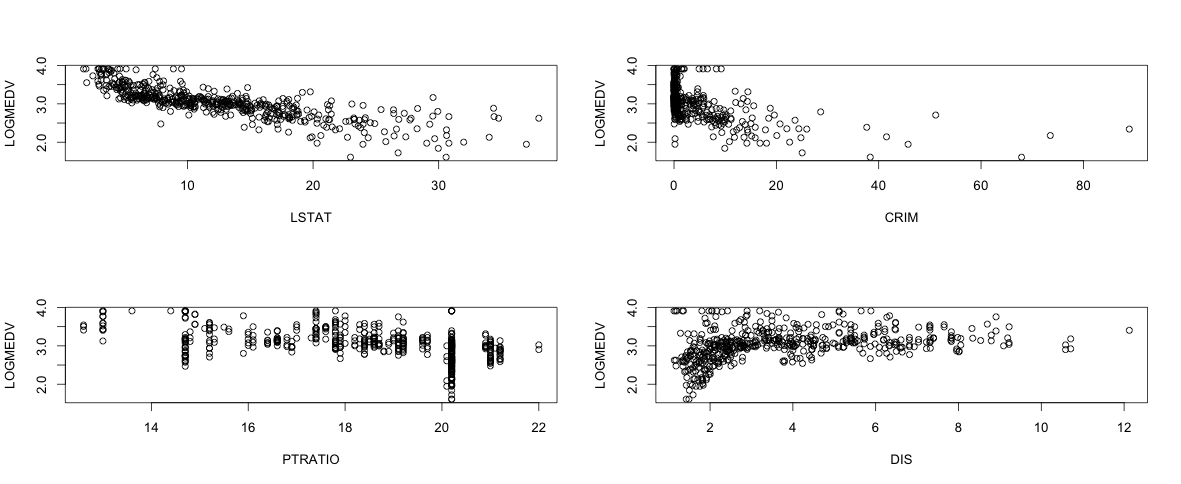
\includegraphics[width=0.9\linewidth]{imagenes/variables_relevantes}
\caption{Variables más relevantes del modelo lineal}
\label{fig:variables_relevantes}
\end{figure}

Vemos que cuanto más bajo es el porcentaje de clase baja, el valor de las casas es mayor. En el caso del crimen, el valor de las casas es mayor cuanto menos crimen hay. En el caso del ratio alumno-profesor, cuanto mayor es el valor de las casas, menor es el ratio alumno-profesor. Por último, cuanto mayor es el valor de las casas, mayor es la distancia a centros de empleo.\\

Calculamos la distribución conjunta a posteriori de $\beta$ y $\sigma$. La Figura~\ref{fig:histograma_beta} muestra los histogramas de los coeficientes $\beta_i$ y la desviación estándar a posteriori.

\begin{figure}[tbph!]
\centering
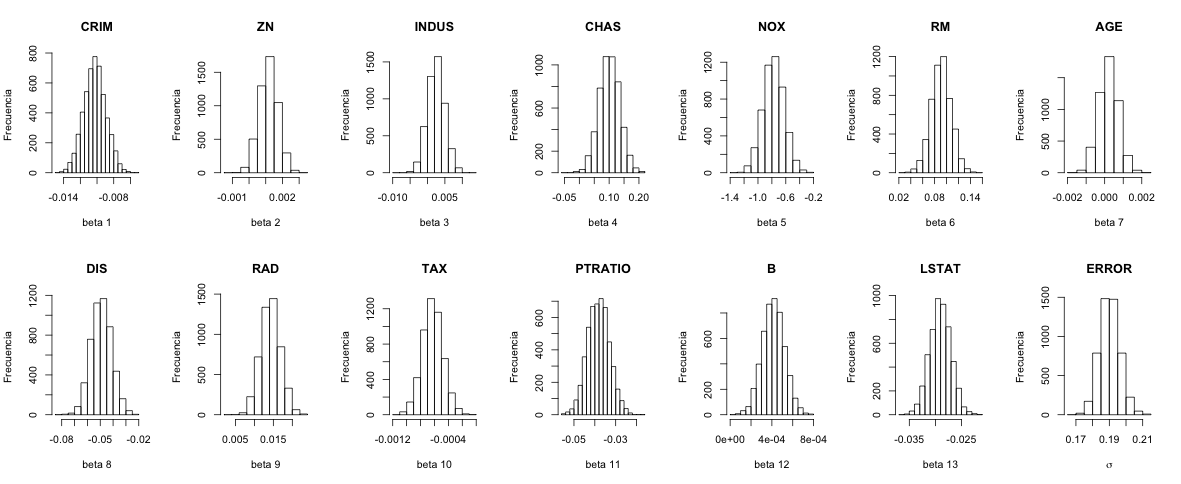
\includegraphics[width=0.9\linewidth]{imagenes/histograma_beta}
\caption{Histograma de los coeficientes $\beta_i$ y la desviación estándar a posteriori}
\label{fig:histograma_beta}
\end{figure}

Calculamos los percentiles 5, 50 y 95 de cada parámetro del modelo lineal ($\beta$ y $\sigma$) . Para cada $\beta_i$ son los siguientes:

\begin{verbatim}
    X(Intercept)        XCRIM          XZN       XINDUS      XCHAS
5%      3.774508 -0.012409392 0.0002397377 -0.001546935 0.04536597
50%     4.101824 -0.010275002 0.0011665871  0.002396406 0.10146128
95%     4.436175 -0.008135323 0.0020905808  0.006668220 0.15781939

            XNOX        XRM          XAGE        XDIS        XRAD    
5%    -1.0349746 0.06376497 -0.0006742242 -0.06235639 0.009770426 
50%   -0.7789356 0.09074896  0.0001967401 -0.04922668 0.014234135
95%   -0.5268495 0.11861673  0.0010928985 -0.03593865 0.018509219

              XTAX    XPTRATIO           XB      XLSTAT
5%   -0.0008676581 -0.04668706 0.0002355121 -0.03236402
50%  -0.0006270491 -0.03829977 0.0004124994 -0.02902430
95%  -0.0003784013 -0.02951471 0.0005861068 -0.02565000
\end{verbatim}

Y para $\sigma$, los valores son los siguientes:

\begin{verbatim}
       5%       50%       95% 
0.1809709 0.1901171 0.2006010 
\end{verbatim}

Supongamos que estamos interesados en comprobar cuál es el valor esperado de las casas en las que las vías cruzan el río y no lo cruzan. Para ello, creamos un grupo de covariables de la siguiente forma: todas las variables, excepto CHAS, tendrán el valor mediano de sus variables, y para CHAS usaremos sus dos valores: 0 y 1. Es decir, las covariables quedan de la siguiente manera:

\begin{table}[htbp!]
\centering
\resizebox{\textwidth}{!}{%
\begin{tabular}{cccccccccccccc}
\hline
Covariable & CRIM   & ZN     & INDUS  & NOX    & RM     & AGE     & DIS    & RAD    & TAX      & PTRATIO & B        & LSTAT   & CHAS \\ \hline
A          & 0.2565 & 0.0000 & 9.6900 & 0.5380 & 6.2085 & 77.5000 & 3.2075 & 5.0000 & 330.0000 & 19.0500 & 391.4395 & 11.3600 & 0    \\ \hline
B          & 0.2565 & 0.0000 & 9.6900 & 0.5380 & 6.2085 & 77.5000 & 3.2075 & 5.0000 & 330.0000 & 19.0500 & 391.4395 & 11.3600 & 1    \\ \hline
\end{tabular}
}
\end{table}

Usamos R para obtener el valor medio de cada covariable (Figura~\ref{fig:esperado}). Observamos que apenas existen diferencias entre el valor de las casas si las vías cruzan el río o no, lo que pone de manifiesto la poca importancia que tiene esta variable en el modelo.\\

\begin{figure}[tbph!]
\centering
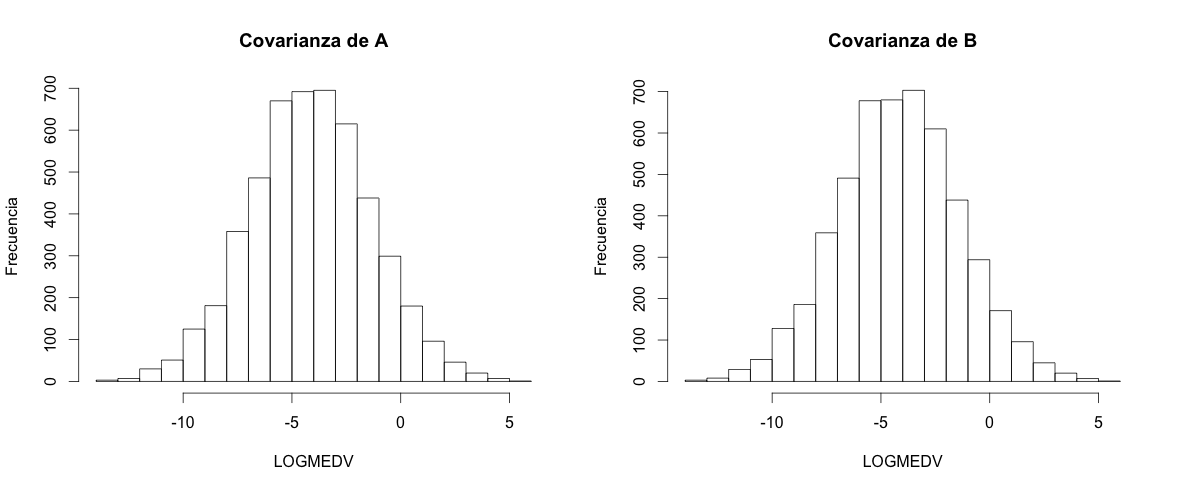
\includegraphics[width=0.9\linewidth]{imagenes/esperado}
\caption{Histograma del valor medio esperado de las covariables}
\label{fig:esperado}
\end{figure}

Si ahora predecimos el valor de las casas de las covariables (Figura~\ref{fig:predecido}), vemos que la diferencia de valor de las casas entre covariables no es apreciable.\\

\begin{figure}[tbph!]
\centering
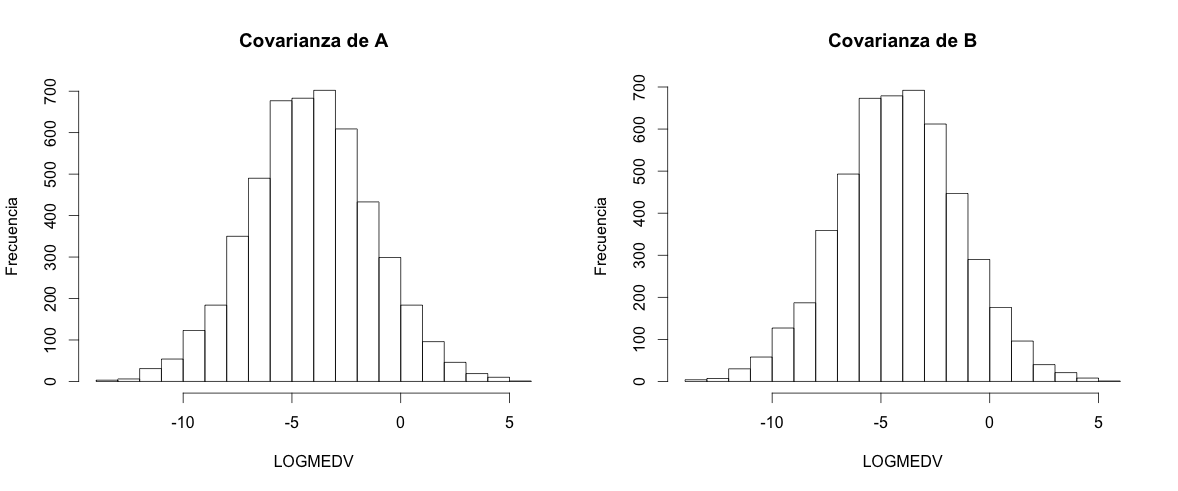
\includegraphics[width=0.9\linewidth]{imagenes/predecido}
\caption{Histograma del valor medio predecido de las covariables}
\label{fig:predecido}
\end{figure}

Por último, calculamos los residuos bayesianos del modelo obtenido. En la Figura~\ref{fig:outliers} observamos que existen 30 valores de casas, con probabilidad mayor que 0.4, que no están bien explicada por el resto de las variables de este modelo. El valor que se indica en el gráfico es el valor medio de la casa (en miles de dólares).\\

\begin{figure}[tbph!]
\centering
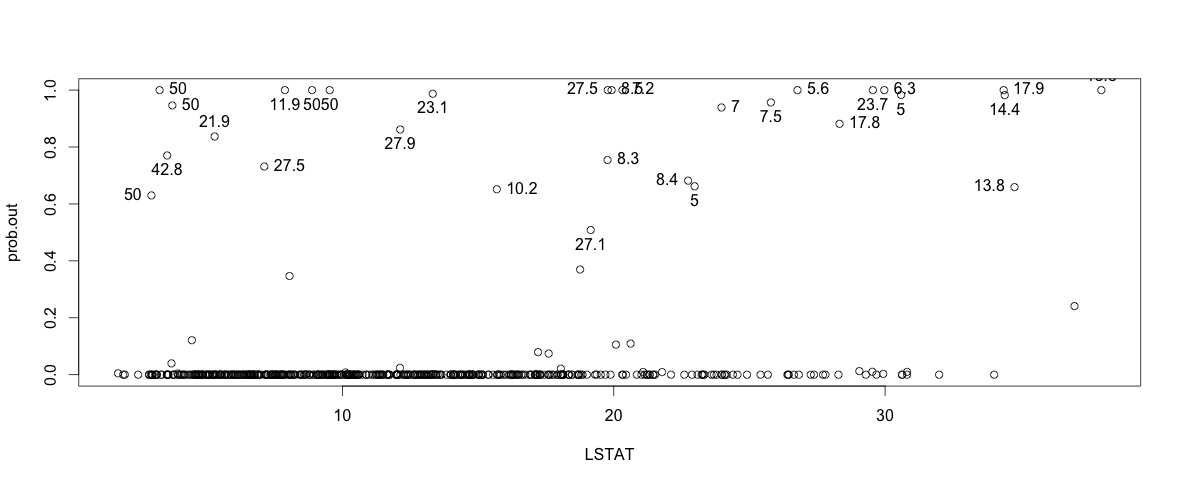
\includegraphics[width=0.9\linewidth]{imagenes/outliers}
\caption{Probabilidades de los outliers frente a la variable LSTAT}
\label{fig:outliers}
\end{figure}

\section{Conclusiones}

En este caso práctico hemos aprendido a usar modelos lineales con R, y en particular, para predecir el valor de las casas a partir de otras variables como la tasa el crimen o el ratio alumno-profesor. En nuestro modelo, casi todas las variables eran predictoras, excepto dos que apenas aportaban al modelo. Las variables más influyentes eran el crimen, el porcentaje de clase baja, el ratio alumno-profesor y la distancia a centros de empleo, entre otras. Aplicando transformaciones a los datos, hemos obtenido mejoras con respecto a nuestro modelo inicial. Por último, usando R ahorramos bastante tiempo debido al gran número de funciones y librerías,  y su potencia de cálculo.

\newpage

\section{Código R}

\verbatiminput{../caso_iv.R}


\end{document} 